\begin{figure}%[ht]
\centering

% \subfloat[The reduction for the example \autoref{example_ECD}.\label{fig:example_graph_reduction}]%{0.3\textwidth}
%     {\begin{tikzpicture}[scale=0.5, auto, swap]

%         % Nodes in C (Coupons)
%         \node[draw, circle] (A) at (0, 2) {A};
%         \node[draw, circle] (B) at (0, 0.5) {B};
%         \node[draw, circle] (C) at (0, -1) {C};
%         \node[draw, circle] (D) at (0, -2.5) {D};
%         \node[draw, circle] (E) at (0, -4) {E};

%         % Nodes in V (Values)
%         \node[draw, circle] (v1) at (3, 2) {$\ell _1$};
%         \node[draw, circle] (v2) at (3, 0.5) {$\ell _2$};
%         \node[draw, circle] (v3) at (3, -1) {$\ell _3$};
%         \node[draw, circle] (v4) at (3, -2.5) {$\ell _4$};
%         \node[draw, circle] (v5) at (3, -4) {$\ell _5$};
        
%         % Draw edges (samples)
%         \draw[-] (A) -- (v1);
%         \draw[-] (B) -- (v2);
%         \draw[-] (C) -- (v3);
%         \draw[-] (D) -- (v4);
%         \draw[-] (E) -- (v5);

%         % Labels above the nodes
%         \node at (-0.5, 3.2) {Coupons ($C$)};
%         \node at (3.5, 3.2) {Values ($V$)};
%     \end{tikzpicture}
% }
%     \hfill
% \hspace{0.05\textwidth} % Horizontal space between the figures
%\subfloat[Reduction of the Coupon Collector’s Problem to a Bipartite Graph.\label{fig:graph_reduction}]{
%     \centering
%     \begin{tikzpicture}[scale=0.5, auto, swap]

%     % Nodes in C (Coupons)
%     \node[draw, circle] (c1) at (-5, 2) {$c_1$};
%     \node[draw, circle] (ci) at (-2, 2) {$c_i$};
%     \node[draw, circle] (cj) at (1, 2) {$c_j$};
%     \node[draw, circle] (cn) at (4, 2) {$c_n$};
%     \node[draw, circle] (ck) at (-7, 4) {$c_k$}; % New coupon node
%     \node[draw, circle] (cl) at (6, 3) {$c_l$}; % New coupon node

%     % Nodes in V (Values)
%     \node[draw, circle] (v1) at (-5, -2) {$\ell _1$};
%     \node[draw, circle] (vi) at (-2, -2) {$\ell _i$};
%     \node[draw, circle] (vj) at (1, -2) {$\ell _j$};
%     \node[draw, circle] (vn) at (4, -2) {$\ell _n$};
%     \node[draw, circle] (vm) at (-6, -4) {$\ell _m$}; % New value node
%     \node[draw, circle] (vo) at (7, -3) {$\ell _o$}; % New value node

%     % Dots for indicating more nodes
%     \node[scale=0.75] at (-3.5, 2) {$\cdots$};
%     \node[scale=0.75] at (-3.5, -2) {$\cdots$};
%     \node[scale=0.75] at (-0.5, 2) {$\cdots$};
%     \node[scale=0.75] at (-0.5, -2) {$\cdots$};
%     \node[scale=0.75] at (2.5, 2) {$\cdots$};
%     \node[scale=0.75] at (2.5, -2) {$\cdots$};

%     % Edges (Samples)
%     \draw[-] (c1) -- (vi);
%     \draw[-] (ci) -- (vj);
%     \draw[-] (cn) -- (v1);
%     \draw[-] (cj) -- (vn);
%     \draw[-] (ck) -- (vj); % New edge
%     \draw[-] (cl) -- (vm); % New edge
%     \draw[-] (c1) -- (vo); % New edge crossing existing edge
%     \draw[-] (vn) -- (ck); % New edge crossing existing edge

%     % Labels above the nodes
%     \node at (0, 5) {Coupons ($C$)};
%     \node at (0, -5) {Labels ($V$)};
    
% \end{tikzpicture}
% }

    \centering
    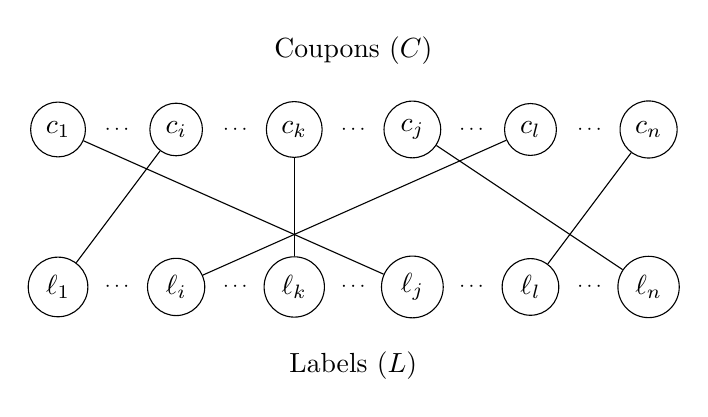
\begin{tikzpicture}[scale=0.5, auto, swap]
    
        % Nodes in C (Coupons)
        \node[draw, circle] (c1) at (-9, 2) {$c_1$};
        \node[scale=0.75] at (-7.5, 2) {$\cdots$};
        \node[draw, circle] (ci) at (-6, 2) {$c_i$};
        \node[scale=0.75] at (-4.5, 2) {$\cdots$};
        \node[draw, circle] (ck) at (-3, 2) {$c_k$};
        \node[scale=0.75] at (-1.5, 2) {$\cdots$};
        \node[draw, circle] (cj) at (0, 2) {$c_j$};
        \node[scale=0.75] at (1.5, 2) {$\cdots$};
        \node[draw, circle] (cl) at (3, 2) {$c_l$};
        \node[scale=0.75] at (4.5, 2) {$\cdots$};
        \node[draw, circle] (cn) at (6, 2) {$c_n$};
    
        % Nodes in V (Values)
        \node[draw, circle] (v1) at (-9, -2) {$\ell _1$};
        \node[scale=0.75] at (-7.5, -2) {$\cdots$};
        \node[draw, circle] (vi) at (-6, -2) {$\ell _i$};
        \node[scale=0.75] at (-4.5, -2) {$\cdots$};
        \node[draw, circle] (vk) at (-3, -2) {$\ell _k$};
        \node[scale=0.75] at (-1.5, -2) {$\cdots$};
        \node[draw, circle] (vj) at (0, -2) {$\ell _j$};
        \node[scale=0.75] at (1.5, -2) {$\cdots$};
        \node[draw, circle] (vl) at (3, -2) {$\ell _l$};
        \node[scale=0.75] at (4.5, -2) {$\cdots$};
        \node[draw, circle] (vn) at (6, -2) {$\ell _n$};
    
        % Edges (Perfect Matching)
        \draw[-] (c1) -- (vj);
        \draw[-] (cn) -- (vl);
        \draw[-] (ci) -- (v1);
        \draw[-] (cj) -- (vn);
        \draw[-] (cl) -- (vi);
        \draw[-] (ck) -- (vk);
    
        % Labels above the nodes
        \node at (-1.5, 4) {Coupons ($C$)};
        \node at (-1.5, -4) {Labels ($L$)};
        
    \end{tikzpicture}
    
    %The coupons \(c_i\) are connected to their corresponding values \(\ell _j\) through edges representing the values' matching.}

\caption{\footnotesize
CCP by collecting edges in a bipartite graph. The coupons (\(C\)) are matched to the labels (\(L\)) via edges, representing samples. This graph-based representation highlights the CCP as a problem of reconstructing all edges with minimal sampling.\label{fig:graph_reduction}
% OR
% A visualization of the reduction of the CCP to a bipartite graph structure. Nodes in the top row (\(C\)) represent coupons, while nodes in the bottom row (\(L\)) represent the labels they can be matched to. Each edge between \(c_i \in C\) and \(\ell _j \in L\) corresponds to a sample where the value \(\ell _j\) is observed for the coupon \(c_i\). The bipartite graph representation enables studying the CCP as a graph reconstruction problem, where the goal is to research the number of samples needed to recover all pairwise connections.\label{fig:graph_reduction}
}
\vspace{-4ex}
\end{figure}